\documentclass[10pt]{article}
\usepackage{graphicx} % Required for the inclusion of images
%\usepackage{subcaption}
%\usepackage{subfig}
\usepackage{natbib} % Required to change bibliography style to APA
\usepackage{amsmath} % Required for some math elements 
\usepackage{booktabs}
\usepackage{float}


\title{Assignment 1 report \\ Part A: Experimenting with performance} % Title

\author{Chen Wang, Xiahe Liu (Group 37)} % Author name

\date{\today} % Date for the report

\begin{document}

\maketitle % Insert the title, author and date


% If you wish to include an abstract, uncomment the lines below
% \begin{abstract}
% Abstract text
% \end{abstract}

%----------------------------------------------------------------------------------------
%	SECTION 1
%----------------------------------------------------------------------------------------

\section{Experimental Setup}

For this assignment, we set up 4 Standard D12\_V2 virtual machines (VMs) on Azure, each with 4 cores, 28 GB memory, 50 GB disk and 200 GB temporary disk. We also have hadoop-2.6.0 deployed on each VM, where VM4 works as the master and slave and the rest VMs work as slaves. Tez-0.7.1 and Hive-1.2.1 are deployed on the master VM. For the workload, we generate a 50 GB TPC-DS database, which is stored in HDFS. Specifically, we use query 12, 21, 50, 71 and 85 to verify the performance of Mapreduce and Tez for this assignment. 

%----------------------------------------------------------------------------------------
%	SECTION 2
%----------------------------------------------------------------------------------------

\section{Mapreduce vs. Tez}
In this section, we evaluate the performance of Hive/Mapreduce and Hive/Tez in term of query completion time, bandwidth transmit/receive, disk read/write. Meanwhile, the differences of Mapreduce and Tez can be seen from the task distribution and Directed Acyclic Graph (DAG).

\subsection{Completion time}
We run query 12, 21, 50, 71 and 85 of TPC-DS benchmark set with Hive/Mapreduce and Hive/Tez (for simplicity, we use Mapreduce and Tez for the rest of this report). Figure \ref{fig:q1a_time} represents the completion time of the queries, Tez can achieve shorter completion time for query 12, 21 and 50, however Mapreduce outperforms Tez for query 71 and 85. To obtain the reason behind this, we will show the disk I/O, data transfer between VMs, task distribution and DAG of the queries for the rest of this section. It seem that some heavy disk I/O and data transfer for Tez consume lots of time, lead to longer completion time, such as that of query 71 and 85. On the other hand, the computation structure may influence the completion time as well, Tez with arbitrary DAG can avoid unnecessary intermediate data read/write and gets a much more natural way to translate the computation for some scenarios, like that of query 12 and 21.

\begin{figure}
\begin{center}
\includegraphics[width=0.75\textwidth]{pic/q1a_time}
\caption{Completion Time of MR and Tez (default parameters).}
\label{fig:q1a_time}
\end{center}
\end{figure}


\subsection{Network and Disk}
Figure \ref{fig:q1b_net} shows the data transmitted and received during the query's lifetime. For query 12, 21, 50 and 71, Mapreduce transmits/receives more data through network interface eth0 than Tez does. Especially for query 21, the transmitted and received data is about ten times than that of Tez. However, Tez consumes more network resource than Mapreduce for query 85.

\begin{figure}
\begin{center}
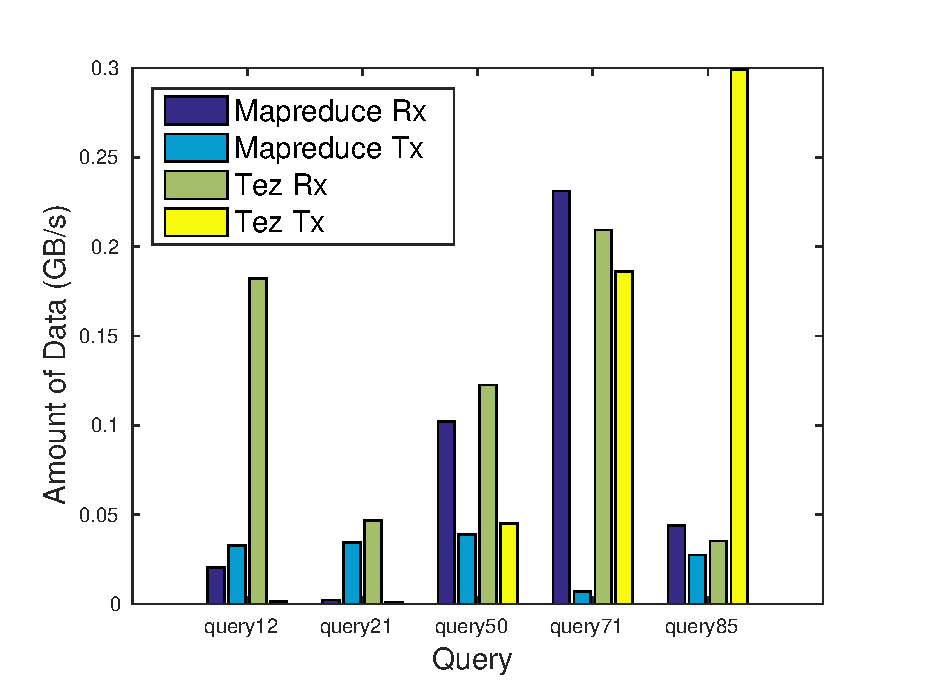
\includegraphics[width=0.75\textwidth]{pic/q1b_net}
\caption{Bandwidth Consumption of MR and Tez (default parameters).}
\label{fig:q1b_net}
\end{center}
\end{figure}

Figure \ref{fig:q1b_disk} shows the amount of data written/read to/from HDFS during the query's lifetime. Mapreduce write much more to HDFS than Tez does for query 12 and 21, which could cost a large running time. For query 50, Mapreduce and Tez have similar performance in terms of HDFS read/write. For query 71 and 85, the data read from HDFS is similar for Mapreduce and Tez, however Tez writes about 30 and 17 times of data to HDFS than Mapreduce, respectively, which can be one of the possible causes for longer completion time of query 71 and 85 with Tez. And it's known that remote disk write/read can be costly.

\begin{figure}
\begin{center}
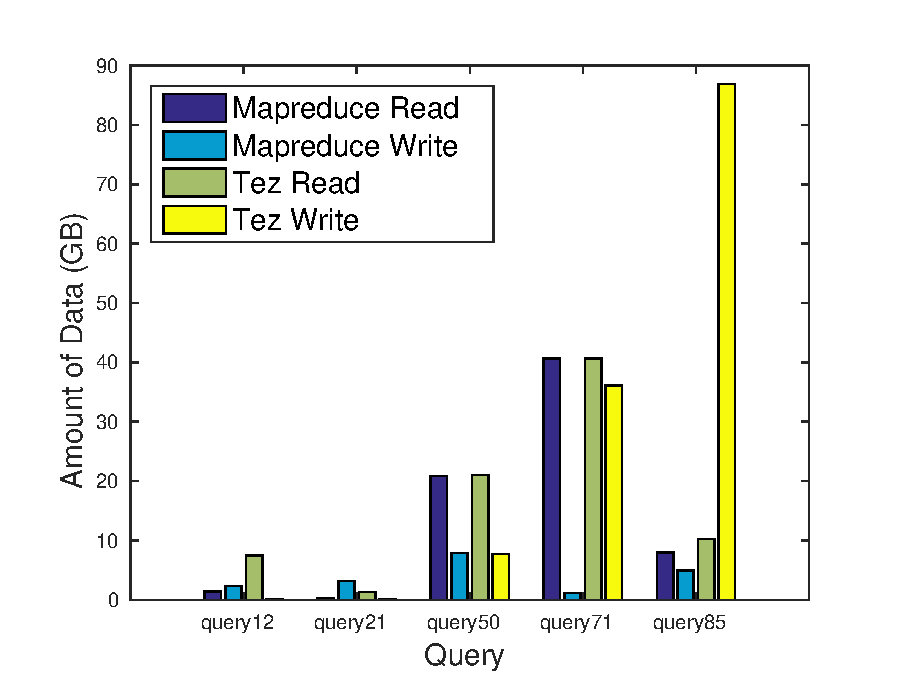
\includegraphics[width=0.75\textwidth]{pic/q1b_disk}
\caption{Disk I/O of MR and Tez (default parameters).}
\label{fig:q1b_disk}
\end{center}
\end{figure}

\subsection{Tasks}

For the total number of tasks for each query, Tez utilizes more tasks than Mapreduce for query 12, 21 and 50. For Mapreduce, query 12, 21 and 71 have more than 90\% of their tasks to aggregate data, while the numbers of aggregate tasks and HDFS read tasks are much closer for query 50 and 85, which can be seen from Table \ref{tab:mr_agg_task}. Table \ref{tab:tez_agg_task} shows the aggregate tasks, HDFS read tasks and total tasks of Tez for different queries. We can observe that Tez also uses  most of the tasks to read data from HDFS for query 12 and 21. Different from that of Mapreduce, Tez only has about 5\% tasks for aggregating for query 50. But for query 71 and 85, most of the tasks are working for aggregating from HDFS. 

\begin{table}[htbp]
  \centering
  \caption{The Number of Aggregate Tasks, HDFS Read Tasks and Total Tasks for Mapreduce}
    \begin{tabular}{lccccc}
    \toprule
    Query ID & 12    & 21    & 50    & 71    & 85 \\
    \midrule
    \# Total Task & 42    & 22    & 187   & 170   & 92 \\
    \# Aggregate Task & 39    & 20    & 99    & 168   & 52 \\
    Percentage & 92.86\% & 90.91\% & 52.94\% & 98.82\% & 56.52\% \\
    \# HDFS Rea Task & 3     & 2     & 88    & 2     & 40 \\
    Percentage & 7.14\% & 9.09\% & 47.06\% & 1.18\% & 43.48\% \\
    \bottomrule
    \end{tabular}%
  \label{tab:mr_agg_task}%
\end{table}%

\begin{table}[htbp]
  \centering
  \caption{The Number of Aggregate Tasks, HDFS Read Tasks and Total Tasks for Tez}
    \begin{tabular}{lccccc}
    \toprule
    Query ID & 12    & 21    & 50    & 71    & 85 \\
    \midrule
    \# Total Task & 55    & 31    & 97    & 144   & 85 \\
    \# Aggregate Task & 2     & 3     & 5     & 139   & 61 \\
    Percentage & 3.64\% & 9.68\% & 5.15\% & 96.53\% & 71.76\% \\
    \# HDFS Read Task & 53    & 28    & 92    & 5     & 24 \\
    Percentage & 96.36\% & 90.32\% & 94.85\% & 3.47\% & 28.24\% \\

    \bottomrule
    \end{tabular}%
  \label{tab:tez_agg_task}%
\end{table}%


Figure \ref{fig:q1c_tasks_12} shows the task distribution over time for query 12 with Mapreduce and Tez, respectively. For the query with Mapreduce, we can observe 5 stages with idle time slots (e.g. the time period during 38s from 50s). The reason for those idle time slot without tasks could be explained as follows, when the computation of each stage completed, the intermediate results are written back to HDFS, then the tasks for the next stage start to read those results from HDFS. Repeated interactions with HDFS lead to longer completion time due to relatively inefficient disk I/O, meantime, the restricted Map/Reduce translation is unnatural for some scenarios and can cause high overhead. However, Tez eliminates those drawbacks by using a more flexible DAG oriented model instead of the restricted Map/Reduce stages in Mapreduce. As Figure \ref{fig:q1c_tasks_12} shows that the task distribution of Tez is much more stable than that of Mapreduce, which may benefit the total completion time of the job.

\begin{figure}
\begin{center}
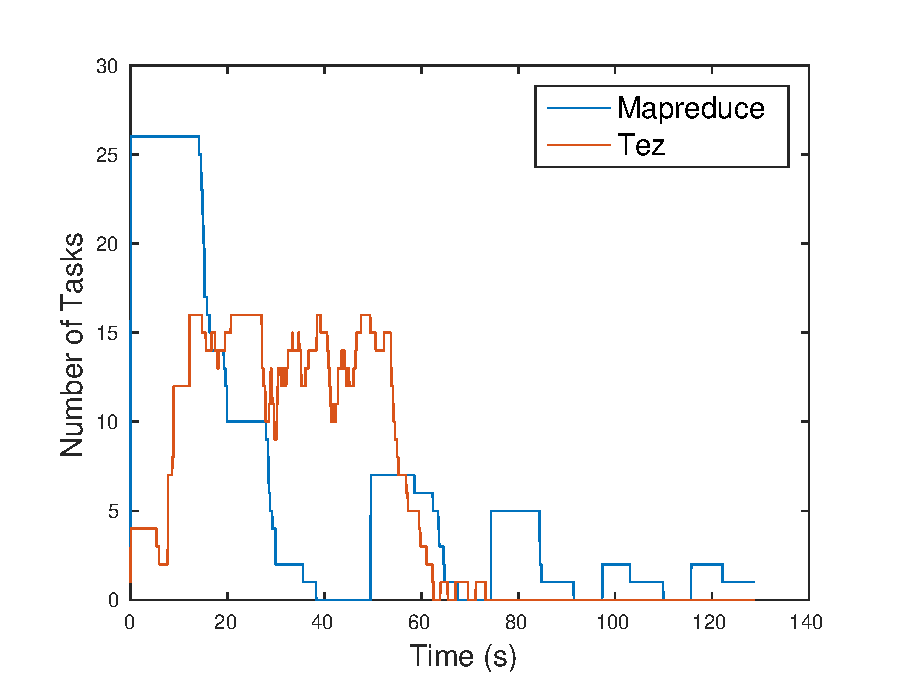
\includegraphics[width=0.75\textwidth]{pic/q1c_task_distribution_12}
\caption{Tasks Distribution over Time (query 12).}
\label{fig:q1c_tasks_12}
\end{center}
\end{figure}

The task distribution of query 21 in Figure \ref{fig:q1c_tasks_21} seems to have similar trend to that of query 12, which also have 5 stages with non-task time periods between stages. With the support of arbitrary DAGs, Tez can avoid unnecessary disk I/O and decomposes the query in an efficient way. As we can see that the completion time of Tez is even shorter than the first stage of Mapreduce.

\begin{figure}
\begin{center}
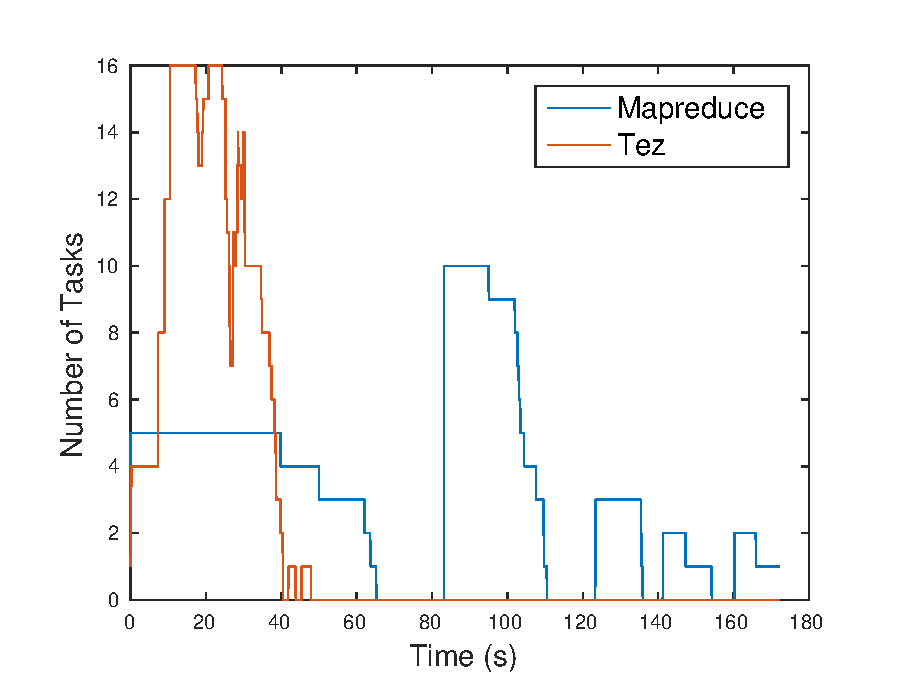
\includegraphics[width=0.75\textwidth]{pic/q1c_task_distribution_21}
\caption{Tasks Distribution over Time (query 21).}
\label{fig:q1c_tasks_21}
\end{center}
\end{figure}

For the task distribution of query 50 in Figure \ref{fig:q1c_tasks_50}, the first stage of Mapreduce can have more than 160 tasks, but the number of tasks decreases over time, then follows with several stages with less than 10 tasks. For Tez, it holds about 16 tasks for the first 150s, after that less than 5 tasks run for about 170s. 

\begin{figure}
\begin{center}
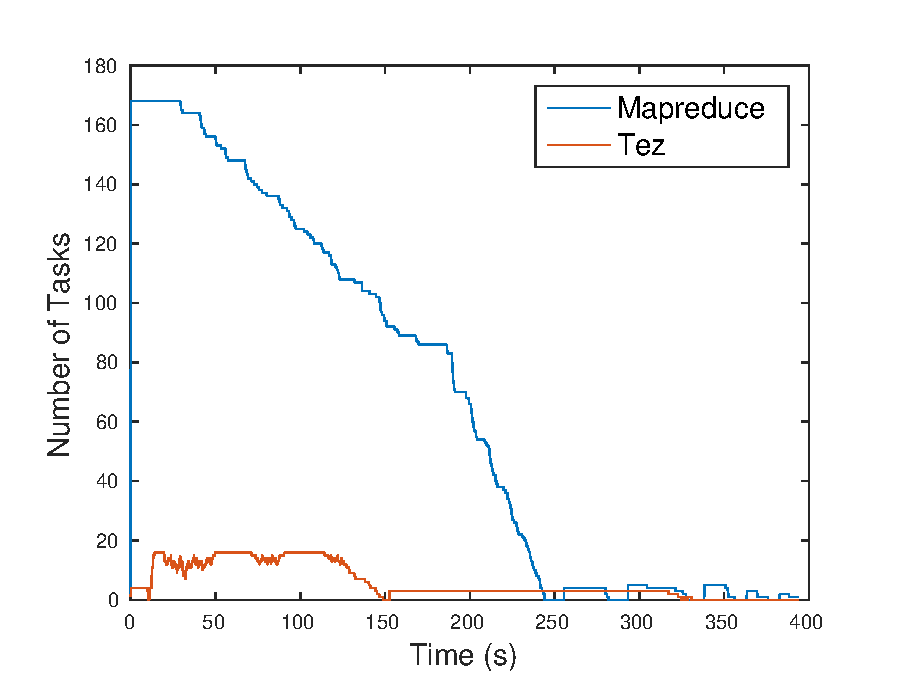
\includegraphics[width=0.75\textwidth]{pic/q1c_task_distribution_50}
\caption{Tasks Distribution over Time (query 50).}
\label{fig:q1c_tasks_50}
\end{center}
\end{figure}

Figure \ref{fig:q1c_tasks_71} presents the task distribution of query 71, similarly, the number of tasks for Tez stays stable without some clear gaps between stages. However, Tez always holds less than or equal to 16 tasks, which might be limited by the resources and configurations. Limited vertexes/tasks and large amount of data read/write makes Tez cost longer time to complete the whole job.

\begin{figure}
\begin{center}
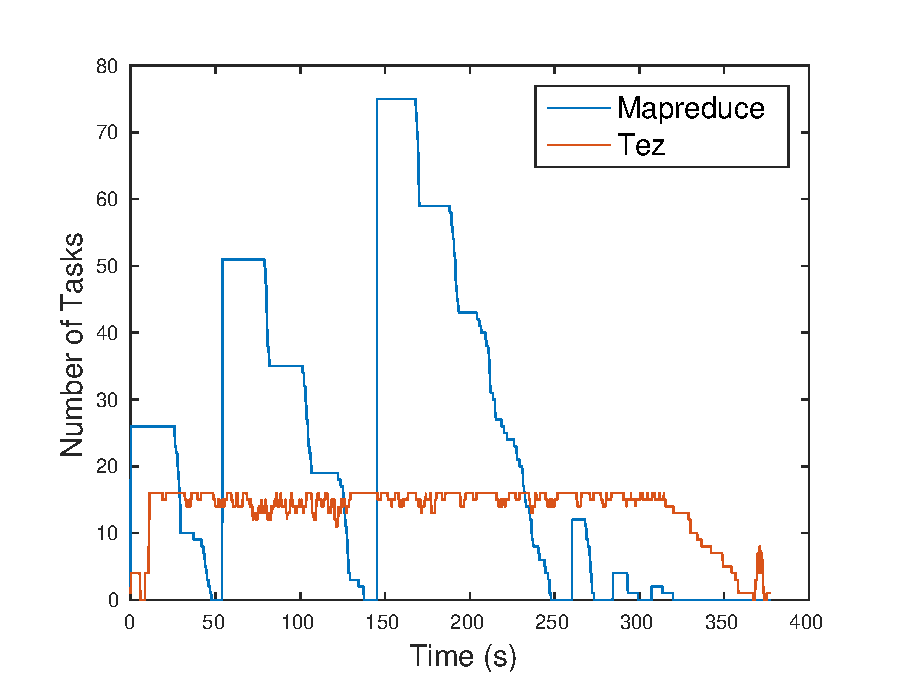
\includegraphics[width=0.75\textwidth]{pic/q1c_task_distribution_71}
\caption{Tasks Distribution over Time (query 71).}
\label{fig:q1c_tasks_71}
\end{center}
\end{figure}

As we mentioned before, the performance of Tez for query 85 is worse than that of Mapreduce, it has longer completion time and more data read/write. From the task distribution in Figure \ref{fig:q1c_tasks_85}, we can obtain that Tez runs about 16 tasks in total for a relatively long time period, similar to that of query 71, noted that we only have 4 virtual machines as slaves, the limited resource and vertexes/tasks can be one of the causes of the bad performance. Differently, Mapreduce has a huge first stage with up to 62 tasks, then a couple of small stages with several tasks followed by, and finally accomplishes the job before Tez does.
\begin{figure}
\begin{center}
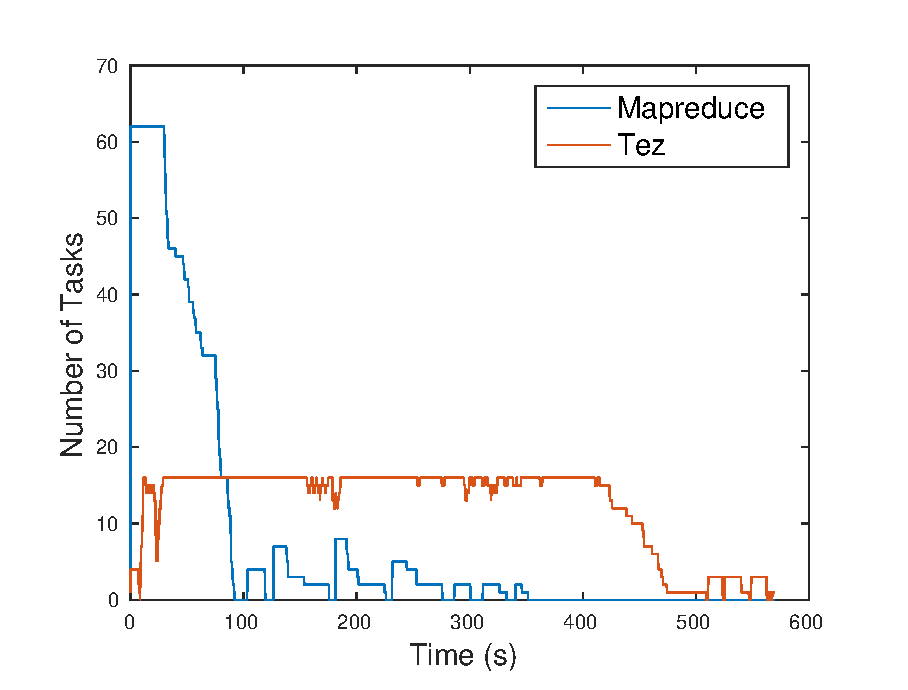
\includegraphics[width=0.75\textwidth]{pic/q1c_task_distribution_85}
\caption{Tasks Distribution over Time (query 85).}
\label{fig:q1c_tasks_85}
\end{center}
\end{figure}


\subsection{Directed Acyclic Graph (DAG)}
In this section, we will show the logic flows of the queries with Mapreduce and Tez. In general, the logic flows after optimization of Mapreduce is simpler than that of Tez, for most queries in this work, it can be a series of sequential Map/Reduce stages. However, the directed acyclic graph (DAG) of Tez is totally different, Tez can build some complicated DAGs with many small stages that are dependent to each other. For instance, the DAGs for query 71 and 85 are two complex ones with complicated dependencies between stages. 

The logic flow of query 12 seems to be straight forward for both Mapreduce and Tez, as Figure \ref{fig:q1d_mr_12} and \ref{fig:q1d_tez_12} show. In Mapreduce, two map only stages followed by three stages with one reducer for each of them. For Tez, two mapper followed by one mapper and three reducers, then the output is written to HDFS, it avoids write/read to/from HDFS for each stage and can be much more efficient. Notice that Mapreduce will write the output to HDFS after each stage, and the next stage will read data from HDFS, and we did not show that on the DAGs of Mapreduce.

\begin{figure}[htbp]
\centering
\begin{minipage}[t]{0.32\textwidth}
\centering
\includegraphics[width=0.32\textwidth]{pic/dag_mr_12}
\caption{Directed Acyclic Graph (DAG) of MR (query 12).}
\label{fig:q1d_mr_12}
\end{minipage}\hfill
\begin{minipage}[t]{0.32\textwidth}
\centering
\includegraphics[width=0.32\textwidth]{pic/dag_mr_21}
\caption{Directed Acyclic Graph (DAG) of MR (query 21).}
\label{fig:q1d_mr_21}
\end{minipage}\hfill
\begin{minipage}[t]{0.32\textwidth}
\centering
\includegraphics[width=0.32\textwidth]{pic/dag_mr_50}
\caption{Directed Acyclic Graph (DAG) of MR (query 50).}
\label{fig:q1d_mr_50}
\end{minipage}
\end{figure}

\begin{figure}[htbp]
\centering
\begin{minipage}[t]{0.48\textwidth}
\centering
\includegraphics[width=0.6\textwidth]{pic/dag_mr_71}
\caption{Directed Acyclic Graph (DAG) of MR (query 71).}
\label{fig:q1d_mr_71}
\end{minipage}\hfill
\begin{minipage}[t]{0.48\textwidth}
\centering
\includegraphics[width=0.6\textwidth]{pic/dag_mr_85}
\caption{Directed Acyclic Graph (DAG) of MR (query 85).}
\label{fig:q1d_mr_85}
\end{minipage}
\end{figure}

\begin{figure}[htbp]
\centering
\begin{minipage}[t]{0.25\textwidth}
  \centering
\includegraphics[width=0.85\textwidth]{pic/dag_tez_12}
\caption{Directed Acyclic Graph (DAG) of Tez (query 12).}
\label{fig:q1d_tez_12}
\end{minipage}\hfill
\begin{minipage}[t]{0.3\textwidth}
\centering
\includegraphics[width=0.85\textwidth]{pic/dag_tez_21}
\caption{Directed Acyclic Graph (DAG) of Tez (query 21).}
\label{fig:q1d_tez_21}
\end{minipage}\hfill
\begin{minipage}[t]{0.4\textwidth}
\centering
\includegraphics[width=0.85\textwidth]{pic/dag_tez_50}
\caption{Directed Acyclic Graph (DAG) of Tez (query 50).}
\label{fig:q1d_tez_50}
\end{minipage}
\end{figure}

\begin{figure}[htbp]
\centering
\begin{minipage}[t]{0.48\textwidth}
  \centering
\includegraphics[width=0.85\textwidth]{pic/dag_tez_71}
\caption{Directed Acyclic Graph (DAG) of Tez (query 71).}
\label{fig:q1d_tez_71}
\end{minipage}\hfill
\begin{minipage}[t]{0.48\textwidth}
\centering
\includegraphics[width=0.85\textwidth]{pic/dag_tez_85}
\caption{Directed Acyclic Graph (DAG) of Tez (query 85).}
\label{fig:q1d_tez_85}
\end{minipage}
\end{figure}


The DAGs for query 21 are quite similar to that of the query 12, a sequence of map/reduce stages for Mapreduce, and a series of Map/Reduce follows three Mappers for Tez, as shown in Figure \ref{fig:q1d_mr_21} and \ref{fig:q1d_tez_21}.

For query 50, Mapreduce has a huge first stage which consists of 82 mappers and 86 reducers and consumes near 250s by observing the task distribution in Figure \ref{fig:q1c_tasks_50}, after that, there are three map only stages and two map/reduce stages. Note that, the intermediate output will be written to HDFS and the next stage read those data from HDFS, similar procedures to other queries with Mapreduce. Tez holds 5 independent map stages for the first step, which can be run in parallel, then there are three reduce stages, after the last reduce stage, it writes the final results back to HDFS, as Figure \ref{fig:q1d_mr_50} and \ref{fig:q1d_tez_50} show.

Figure \ref{fig:q1d_mr_71} represents the optimized DAG query 71 with Mapreduce, there are 3 independent map only stages at first, then a map stage handles the intermediate output from the former three stages, and two map/reduce stages are working to obtain the final results after that. The DAG for query 71 with Tez is more complicated as in Figure \ref{fig:q1d_tez_71}. First of all, there are 5 independent map stages followed by three map stages. Then these three stages will write the output to HDFS, this write operation might be the reason why query 71 with Tez have high disk I/O, high bandwidth consumption and long completion time. A reduce stage also aggregates the output from the three stages mentioned above, and another reduce stage works for the final output.

From Figure \ref{fig:q1d_mr_85}, we can see that query 85 with Mapreduce has a first stage with 30 mappers and 32 reducers, and then 7 map only or map/reduce stages with several mappers/reducers follows in a sequential way. The DAG for query 85 with tez is in Figure \ref{fig:q1d_tez_85}, which contains several map and reduce stages that related to each other, forms a hierarchy structure of stages. The dependencies between stages and heavy disk write in Figure \ref{fig:q1b_disk} might be the causes of long completion time.

%----------------------------------------------------------------------------------------
%	SECTION 3
%----------------------------------------------------------------------------------------

\section{Experiments with Various Parameters}

In this section, we picked up query 21 and varied some specific parameters to verify the performance of Mapreduce and Tez.

\subsection{Hive/MR}
\subsubsection{Number of Reducers}
In this experiment, we varied the number of reducers of MR jobs. For each set of parameters, we ran three times and took the average completion time. The results are shown in Table \ref{tab:num_of_reducers}, the completion time is the shortest when there is only one reducer, and the more reducers the longer completion time for query. To explain this trend, we think that more reducers can lead to complex data transfer operation between mappers and reducers, which may increase the total completion time. However, the differences of completion time for the queries with various number of reducers are only several seconds, which seems to be small. Note that when we ran the query with the same parameters, the completion time gap between different rounds can be more than 10 seconds.

\begin{table}[htbp]
  \centering
  \caption{Number of Reducers and Completion Time}
    \begin{tabular}{rrrrr}
    \toprule
    \# Reducers & 1     & 5     & 10    & 20 \\
    \midrule
    Time (s) & 184.3 & 188.3 & 190.3 & 195.6 \\
    \bottomrule
    \end{tabular}%
  \label{tab:num_of_reducers}%
\end{table}%

\subsubsection{Number of Shuffle Parallel Copies}

This time we tuned the number of parallel transfers during the shuffle phase. Also, for each set we ran 3 times and then took the average value. From Table \ref{tab:num_of_parallel}, we can see there is a trend that with the rising of parallel copies, performance tends to decrease. The query with 10 shuffle parallel copies consumes least time to complete. Still, we need to mention that the number of shuffle parallel copies may not influence the completion time a lot in this experiment.

\begin{table}[htbp]
  \centering
  \caption{Number of Shuffle Parallel Copies and Completion Time}
    \begin{tabular}{rrrrr}
    \toprule
    \# Copies & 5     & 10    & 15    & 20 \\
    \midrule
    Time (s) & 184.3 & 183.8 & 186.6 & 188.5 \\
    \bottomrule
    \end{tabular}%
  \label{tab:num_of_parallel}%
\end{table}%



\subsubsection{Value of Slow Start}

Then, we tried different values on slow start property. From Table \ref{tab:val_of_slow}, we can tell that when the slow start is 0.75, it has the best performance and it is better than the default value 1.

\begin{table}[htbp]
  \centering
  \caption{Value of Slow Start and Completion Time}
    \begin{tabular}{crrrrr}
    \toprule
    Value of Slow Start & 0.05  & 0.25  & 0.5   & 0.75  & 1 \\
    \midrule
    Time (s) & 186.4 & 185.7 & 185.5 & 182.5 & 183.8 \\
    \bottomrule
    \end{tabular}%
  \label{tab:val_of_slow}%
\end{table}%


 

\subsection{Hive/Tez}
\subsubsection{Container Reuse}
With other parameters default, the experiment without container reuse costs 58.23s to complete, and when we enabled container reuse, it takes 50.36s in average. This indicates that reusing containers can avoid some overhead of container initialization and removal, thus can improve the overall performance of Tez.

\subsubsection{Number of Shuffle Parallel Copies}

This time, we tuned the number of shuffle parallel copies on Tez jobs. 3 Times for each set and completion time is on average. Results are shown in Table\ref{tab:num_shuffle_parallel_tez}. For Tez, we actually cannot tell there is a trend for performance with the variance of number of shuffle parallel copies. The completion time of them are quite similar with each other. 

\begin{table}[htbp]
  \centering
  \caption{Number of Shuffle Parallel Copies and Completion Time for Tez}
    \begin{tabular}{rrrrr}
    \toprule
    \# Copies & 5     & 10    & 15    & 20 \\
    \midrule
    Time (s) & 50.36 & 50.7  & 51.81 & 50.57 \\
    \bottomrule
    \end{tabular}%
  \label{tab:num_shuffle_parallel_tez}%
\end{table}%


\subsection{Are the Best Parameters for Query 21 Still Best for Query 12 and 50?}

\subsubsection{Hive/MR}

The best parameters for MR job Query 21 is reducers = 1, parallel copies = 10, slow start = 0.75. After we applied these parameters on Query 12, the average completion time is 178.044 seconds, which is greater than what we got from part 1 experiments with the default settings, 143.804 seconds. After we applied these parameters on Query 50, the average completion time is 571.969 seconds, which is also greater than what we got from part 1 experiments with the default settings, 409.411 seconds. Thus, we can tell that it is not the best for Query 12 and 50. Different queries may have different map/reduce stages, and the best parameter set may not suit other queries.

% % TODO rational

\subsubsection{Hive/Tez}

The best parameters for Tez job Query 21 is reducers = 1, parallel copies = 5, which is happens to be the default settings. After we applied these parameters on Query 12, the average completion time is 72.065 seconds, which is greater than what we got from reducers = 1, parallel copies = 10, 58.263 seconds. After we applied these parameters on Query 50, the average completion time is 320.048 seconds, which has better performance among other parameters we tried. (326.696 seconds for reducers = 1, copies = 10; 326.113 seconds for reducers = 1, copies = 15; 349.039 seconds for reducers = 1, copies = 20). Thus, we can tell that it is not the best for Query 12, but best for Query 50.

% % TODO rational


%----------------------------------------------------------------------------------------
%	SECTION 4
%----------------------------------------------------------------------------------------
\section{Experiments with Slave Failure}
\subsection{Completion Time}

~~~~~This time we compare the performance for MR and Tez, with one DataNode fails at the time of 25 \% completion and 75 \% completion. From Figure \ref{fig:q3a_time}, we can tell that comparing to the completion time of no failure occurs, one DataNode failure leads to the increase of the completion time. And, it is even more expensive if the failure takes place earlier. As shown in Figure \ref{fig:q3a_time}, failure at 25 \% completion makes the completion time much longer than failure at 75 \% completion. This scenario can be explained if when we kill a DataNode at 25 \% completion, some intermediate data was lost or some HDFS read tasks are disrupted, then it may take some time to recovery the data or process. When kill a DataNode at 75 \% completion, if the tasks are working for aggregating/computation, the DataNode failure of HDFS can have less influence than that of at 25 \% completion. But it may still longer the total completion time.


\begin{figure}
\begin{center}
\includegraphics[width=0.85\textwidth]{pic/q3a_time}
\caption{Completion Time of MR and Tez with Failure (query 71).}
\label{fig:q3a_time}
\end{center}
\end{figure}


%----------------------------------------------------------------------------------------
%	BIBLIOGRAPHY
%----------------------------------------------------------------------------------------

%\bibliographystyle{apalike}

%\bibliography{sample}

%----------------------------------------------------------------------------------------


\end{document}